\chapter{Data}
\label{chap:data}
The data used for the analysis of the brain are Magnetic Resonance Imaging (MRI) scans. This type of scanning is often used as it captures the structure of the brain without the need for exposing the patient to radiation (in contrast to X-ray).  

\section{MRI Images}
\label{sec:MRI}

MRI scans are interested in detecting hydrogen in the body. In fact, this element is widely present in water and fat which makes it interesting in order to analyze the inner workings of the human body.
\begin{wrapfigure}{r}{0.6\textwidth}
 \centering
 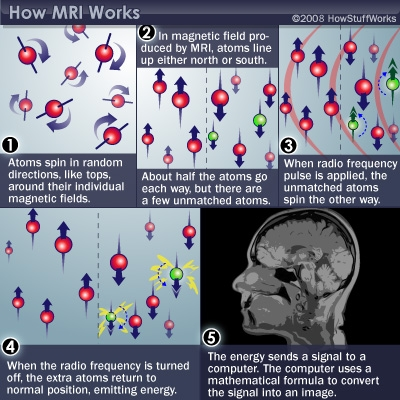
\includegraphics[width=.9\linewidth]{figures/dataset/mri-steps.jpg}
 \captionsetup{width=.9\linewidth}
 \caption[bla]{Steps to acquire an MR Image. Credit howstuffworks.com\footnotemark}
 \label{fig:IXI_hospital_count}
\end{wrapfigure}
\footnotetext{\href{https://science.howstuffworks.com/mri3.htm}{https://science.howstuffworks.com/mri3.htm}}

In normal state protons inside the hydrogen nucleus are spinning in a random direction, but when placed into a strong magnetic field (usually between 0.2 and 3 teslas which is about 10’000 times stronger than magnet people usually use on their fridge). They will align their spin with the field.

Approximately half of them will end up facing the field and the other half in the same direction as the field. In fact, a few more protons will line up their spin in a low configuration. These extra protons, despite being only a few, are the interesting ones.

The second phase consists of sending a specific radio frequency (RF) pulse. The extra protons currently in low-energy configuration will absorb this pulse and flip on their axes. When the RF pulse is stopped, the protons will return into their low-energy configuration and doing so emit RF waves. As different tissues of the brain contain different hydrogen density, this map highlights the different tissues of a brain well, especially the white and gray matter.

Some parameters of the machine can be tuned in order to produce different maps (also called modalities). One of the parameters that can be tuned is the amount of time between two pulses are sent. In fact, two of the most often used modalities (T1 and T2) differ by this parameter. For the rest of the report, when talking about MRI we are indeed referring as T1-weighted images.

As shown later, knowing how these images were formed is quite important, when preprocessing them.

\section{Datasets}
This section explains the different datasets used as well as some basic statistics about them.
\subsection{IXI}
IXI dataset consists of approximately 600 MR Images from healthy patients. Each in T1, T2 and PD-weighted modalities, but for our application, we will concentrate on T1-weighted images only. The data has been collected in 3 different hospitals. For each image, we have the age of the patient together with other information such as if the patient is right or left-handed and his sex. As visualized on figure~\ref{fig:IXI_hospital_count}, the scans come from different hospitals. Further analyses as highlighted in figure~\ref{fig:IXI_age_dist_per_hosp} show that there is a bias on age due to data coming from different hospitals. This could let the model learn where the IRM comes from in order to predict the age. For example, by detecting that an IRM comes from the IOP hospital, the model could output an age around 30 years old without being terribly wrong. Of course, as we do not want that, it is important to normalize our data as illustrated by figure~\ref{fig:intensity_normalization} of the preprocessing pipeline.

\begin{figure}
\centering
\begin{minipage}{.5\textwidth}
  \centering
  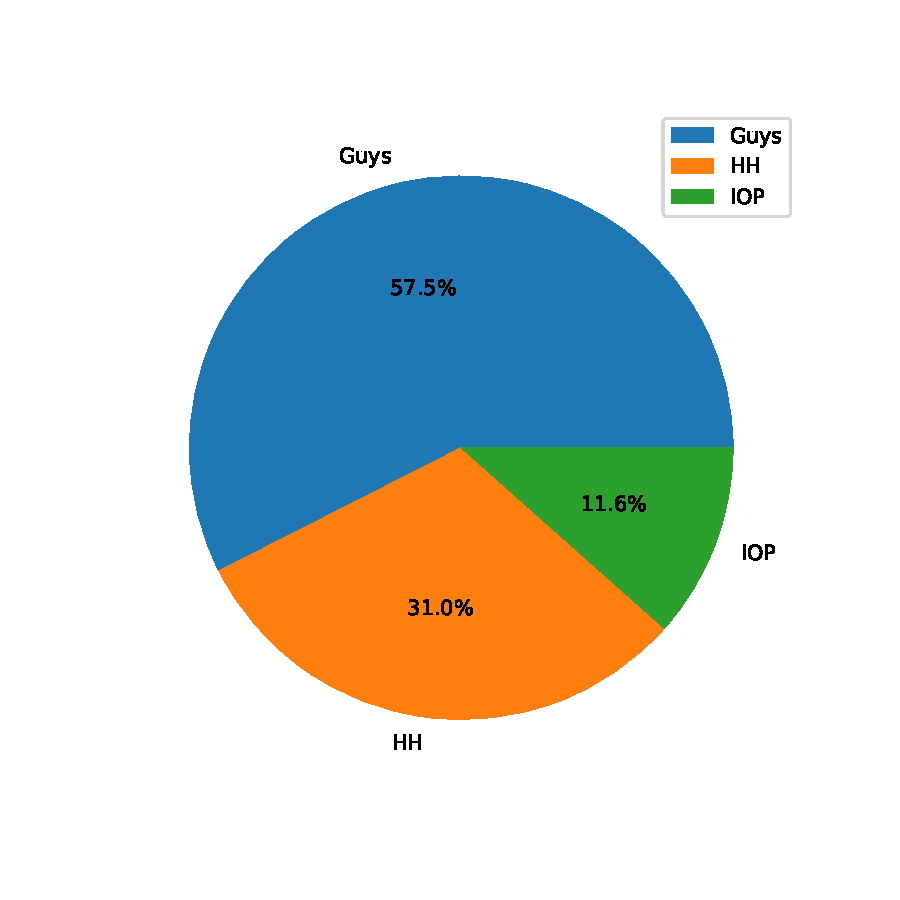
\includegraphics[width=1\linewidth]{figures/dataset/IXI_hospital_count.pdf}
  \captionof{figure}{Scans percentage per hospital.}
  \label{fig:IXI_hospital_count}
\end{minipage}%
\begin{minipage}{.5\textwidth}
  \centering
  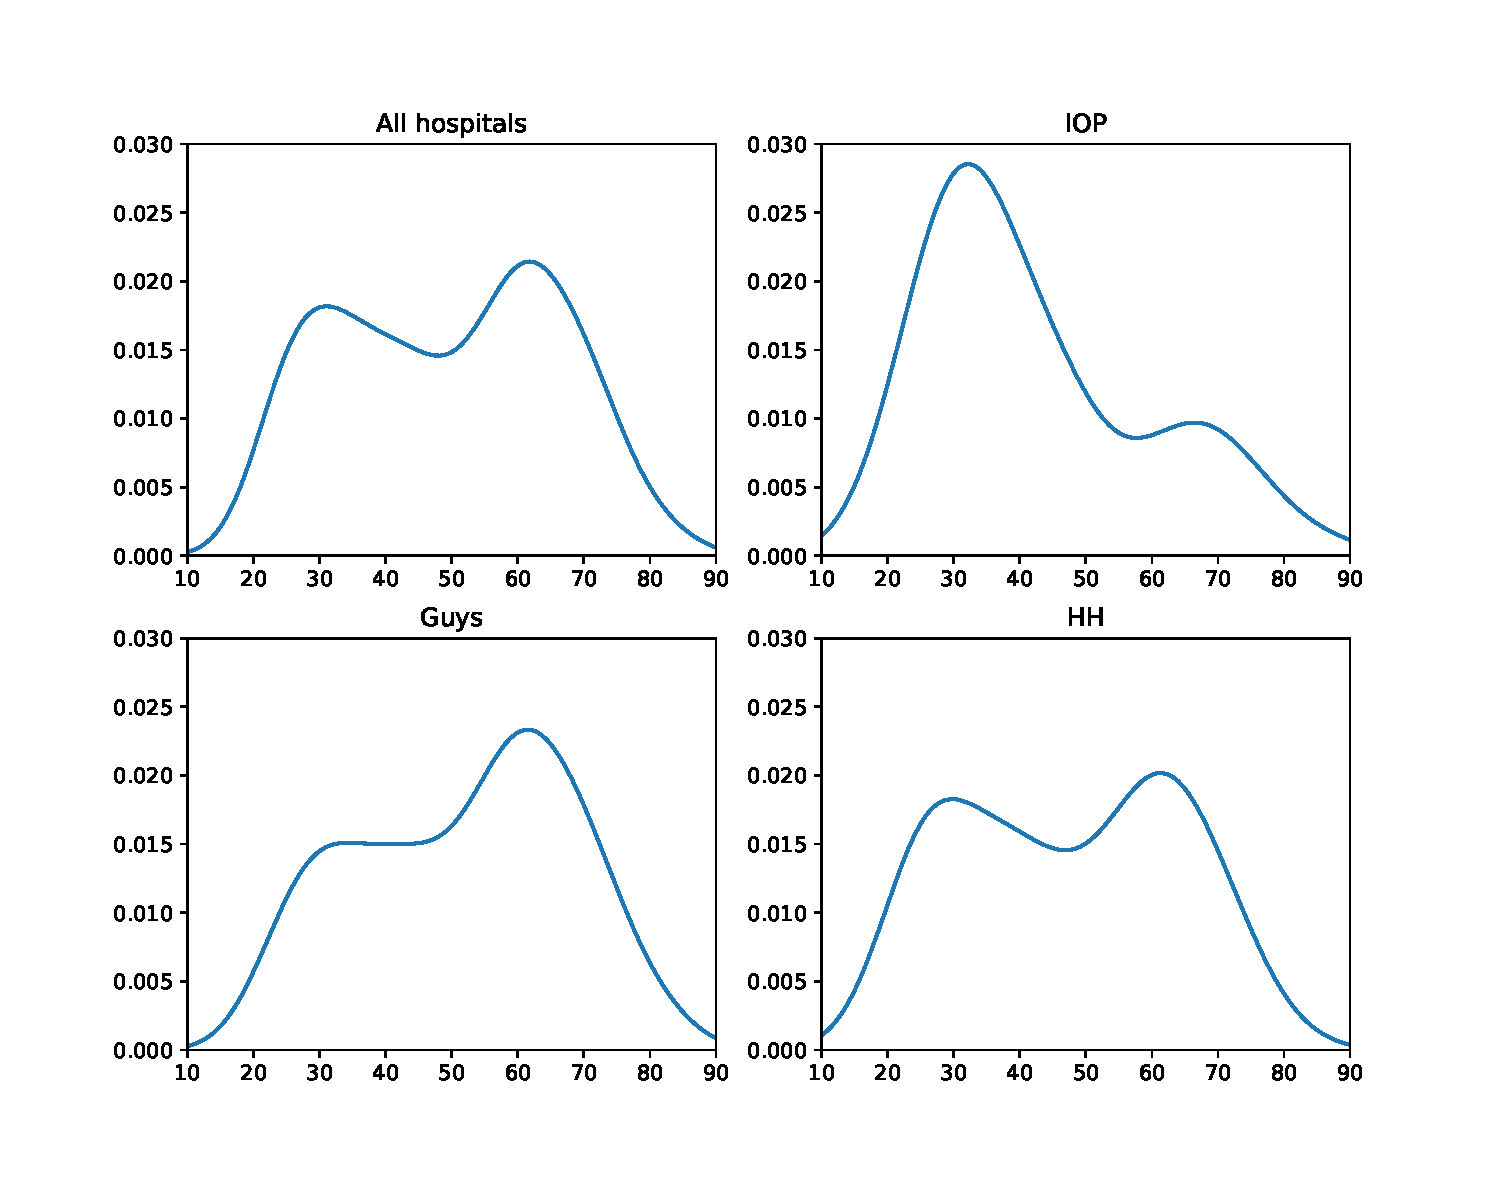
\includegraphics[width=1\linewidth]{figures/dataset/IXI_age_dist_per_hospital.pdf}
  \captionof{figure}{Age distribution for each hospital.}
  \label{fig:IXI_age_dist_per_hosp}
\end{minipage}
\end{figure}

\subsection{OASIS}
\label{sec:OASIS}
This is the main dataset we used in order to train and conduct our analysis of dementia detection and explanation. It consists of 1098 patients for which we can have multiple scans across time. This has to be taken into account when splitting the dataset into train and test sets. If this information is omitted, half scans of a patient could end up in the train set and the other half into the test set, leaking some information between the two sets that are not independent anymore, heading to unreliable evaluation metrics.


Having multiple samples for one patient comes from the longitudinally of the dataset, this influenced the way we attribute labels to a sample. In the dataset, one patient can have multiple diagnoses depending on when he was diagnosed. For example, on the first check up the patient might have been diagnosed healthy, but when checked again 5 years later, his diagnosis might have changed and he might now be classified with dementia. We choose to deal with this situation by taking for each patient his latest (worst) diagnosis as the label for each sample. This choice is motivated by two reasons, firstly we want to build a model that detects dementia as early as possible. Therefore these samples where human failed at making a correct early diagnosis are helping the model into learning features to detect the illness even in situations where the human eye might fail. Secondly, it has been shown by researchers~\cite{change_in_brain_years_before} that the changes in the brain already occur 10 to 20 years before the first symptoms are observed.
\begin{wrapfigure}{l}{0.6\textwidth}
 \centering
 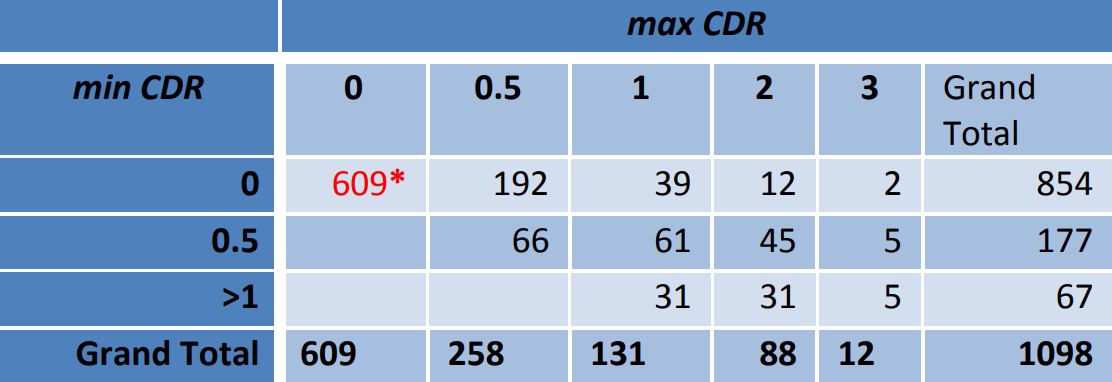
\includegraphics[width=.9\linewidth]{figures/dataset/OASIS_CDR_table.png}
 \captionsetup{width=.9\linewidth}
 \caption[OASIS_CDR_table]{Number of patients per CDR in the OASIS dataset\footnotemark{}.}
 \label{fig:OASIS_CDR_table}
\end{wrapfigure}
\footnotetext{\href{https://www.oasis-brains.org/files/OASIS-3_Imaging_Data_Dictionary_v1.5.pdf}{https://www.oasis-brains.org/files/OASIS-3\_Imaging\_Data\_Dictionary\_v1.5.pdf}}
\begin{wrapfigure}{r}{0.6\textwidth}
 \centering
 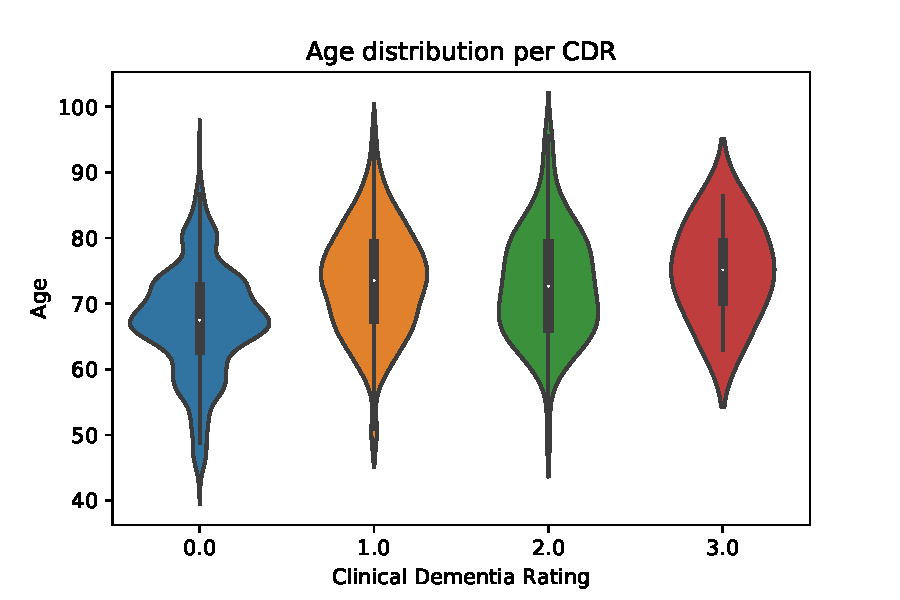
\includegraphics[width=.9\linewidth]{figures/dataset/OASIS_age_dist_per_cdr.pdf}
 \captionsetup{width=.9\linewidth}
 \caption{Distribution of patient age for each class of dementia rating. The width of a violin represents the number of persons for a specific age.}
 \label{fig:OASIS_age_dist}
\end{wrapfigure}

The dataset does not contain a final diagnosis of whether or not a patient has dementia with a certainty of 100 percent. The label associated with each scan is called \textit{clinical dementia rating} (CDR)\footnotemark. This particular diagnosis is based on an interview of both the subject, his caregiver and a clinician. It aimed at testing different cognitive domains such as memory, problem-solving or orientation. The results range from 0 to 3, where 0 stands for no dementia, 0.5 questionable dementia, 1 mild, 2 moderate and 3 severe cognitive impairment. For simplification, we decided to go for only two classes, either dementia or no dementia. Images with CDR 0 are labeled as control image (no dementia) and images with CDR either one two or three were labeled as dement. We choose to discard images with a CDR of 0.5 as these might be confusing for the model. The distribution of CDR can be observed in figure~\ref{fig:OASIS_age_dist}
\footnotetext{\href{https://www.sciencedirect.com/topics/medicine-and-dentistry/clinical-dementia-rating}{https://www.sciencedirect.com/topics/medicine-and-dentistry/clinical-dementia-rating}}

Dementia being often diagnosed for old people, we want to check how this is affecting our dataset. Figure~\ref{fig:OASIS_age_dist} clearly highlights something important about the age distribution in the dataset. We see that dement people tend to be older. To mitigate this effect while training, we build as described in section~\ref{sec:unbias_model} a model that tries to extract features from the image that contains enough information to predict dementia but do not allow the model to predict the age of the patient. 


\section{Preprocessing}
Preprocessing is especially important in medical imaging. For example, a model could easily detect from which hospital/machine the data has been acquired, just by looking at the intensity distribution of voxels if no preprocessing is done. In the case where the data is biased on some hospitals, as it is the case in figure~\ref{fig:IXI_age_dist_per_hosp},  the model could easily overfit on that bias. In fact, due to the expensive price of acquiring data, datasets are often created by merging data from multiple hospital institutes. In addition, we do not want our model to work well on one hospital only, but should generalize as much as possible for other hospitals too. The section below describes in detail the different stage of our preprocessing pipeline to overcome these issues. The overall preprocessing pipeline has been visualize in the figure~\ref{fig:pipeline}.


\subsection{Resampling}
MRI scanners can have different resolutions that directly come from the machine used to acquire the data. To overcome that we use the metadata present in the MRI header to resample the images such that the effective distance between two neighboring voxels is exactly 1mm. This might require a drop of resolution or interpolation in the case where the original image was sampled at a lower resolution.


\subsection{Bias Field Correction}
In medical imaging, one would logically expect that the intensity of a certain type of tissue should always be the same across the image. For example, the value of a voxel representing white matter should be the same independently of its location in the image. However this expectation does not match the reality, there are numerous undesirable artifacts implied by the way the data is recorded. These are often referred to as bias field, and sometimes as shading, intensity non-uniformity/inhomogeneity.  Fortunately for us, this non-uniformity can be assumed to be of low-frequency and thereby to be smooth across the image, which means that it can be estimated and corrected or at least mitigated.
\begin{wrapfigure}{r}{0.5\textwidth}
 \centering
 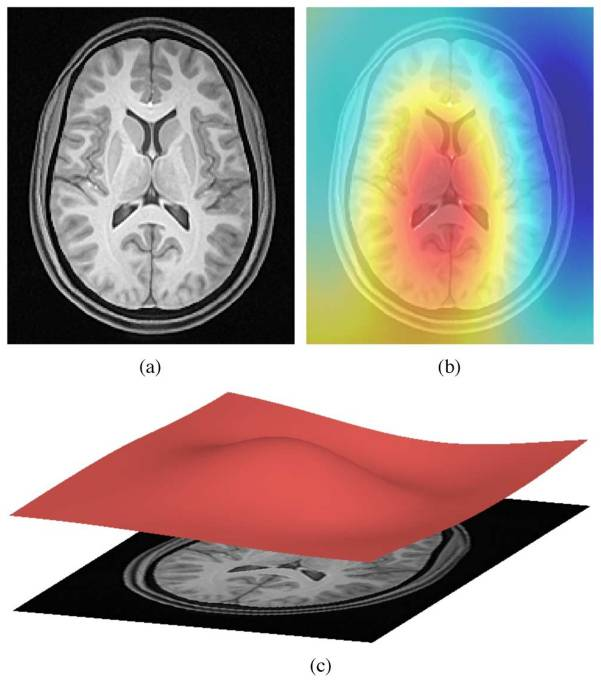
\includegraphics[width=.9\linewidth]{figures/preprocessing/N4_explain.jpeg}
 \captionsetup{width=.9\linewidth}
 \caption[N4]{Bias field correction by N4ITK\footnotemark}
 \label{fig:N4_explain}
\end{wrapfigure}
\footnotetext{\href{https://www.ncbi.nlm.nih.gov/pmc/articles/PMC3071855/}{https://www.ncbi.nlm.nih.gov/pmc/articles/PMC3071855/}}

One can try to correct the bias by modeling the recorded image as a combination of 3 components, the clean image $I$, the bias field of low frequency $B$ and an independent Gaussian noise $\sigma$. This formula is one possible way to combine these components. $S(x,y,z)= I(x,y,z)*B(x,y,z) +\sigma(x,y,z)$. The algorithm we used, assumes that formula, for bias field correction. The low-frequency bias field $B$ can be seen in red in figure~\ref{fig:N4_explain}. It is an improvement over the \textit{non-parametric nonuniform normalization (N3)} and is therefore named N4. 
The exact computation of the bias goes beyond the scope of this thesis, but the reader can find the details in the original paper \cite{N4_paper}.


\subsection{Co-registration}
\label{sec:coregistration}

In the 3D space, the brain can be located anywhere and more precisely rotated or scaled by any factor. As all the models used in this study are based on convolutional layers, it is well known that they can be equivariant or even invariant to translation, but they are not rotation nor scale equivariant. Thus it would greatly help the model to transform the brain scans from all patients so that they are all realigned into a common space. 

Here we chose to align the brain into the MNI152 space\footnotemark{}. The template we used consists of an averaging of 152 healthy brains (healthy subjects) that have been matched using a 9-parameter affine transform. It is commonly used as a standard template. In addition to the averaged brains, this space does provide some useful masks, notably interesting for us a mask of the skull and one of the hippocampus.
\footnotetext{\href{https://fsl.fmrib.ox.ac.uk/fsl/fslwiki/Atlases}{https://fsl.fmrib.ox.ac.uk/fsl/fslwiki/Atlases}}

Some specialists call this process normalization, while co-registration is used to describe the process by which different modalities from the same patient are realigned. That process is slightly easier as the type of transformation between images can be restricted to affine transformation (linear mapping method that preserves points, straight lines, and planes)

Registration can be viewed as an optimization problem formally defined below.
Find $p$ that satisfies
$$\displaystyle  \min_{p} M(I,J, \omega(p))$$
Where $\omega$ is a parametric transformation from a set of allowed transformation. Usually, the metric used to compare the two images is mutual information. The higher the mutual information is between two images the closer they are (similar look).

The algorithm used internally by ANTs\footnotemark{} is the following:
\begin{enumerate}
\item Find the optimal, rigid transform that minimizes the negative Mutual Information.
\item Find the optimal, affine transform that minimizes the negative Mutual Information.
\item Find the optimal diffeomorphism that minimizes the negative Mutual Information.
\end{enumerate}
\footnotetext{\href{https://stnava.github.io/ANTs/}{https://stnava.github.io/ANTs/}}
As only invertible transformations are applied, the resulting output from this algorithm is a register image and an invertible transformation. The fact that the transformation is invertible is quite important as it means that, in total, the information has not been lost but it is now shared between the registered image and the transformation matrix.

Unfortunately, some useful features for the task could now be encoded into the transformation and dealing with the registered image only could lead to bad performances. For this reason, the next steps of the pipeline are going to be executed on both the registered image and the non-registered one. In further work, it would be interesting to train the model on the non-registered image to compare the performances.
 
The optimization task cannot be implemented in one step due to the high number of parameters to tune. Therefore an iterative approach based on the gradient is implemented. This solution might not be the optimal one but does converge towards it. This makes it by far the most computation expensive step of the pipeline, it takes roughly 10 minutes per image to be realigned with the common brain. For that reason, we had to parallelize the preprocessing pipeline using programs such as GNU parallel\footnotemark{}.
\footnotetext{\href{https://www.gnu.org/software/parallel/}{https://www.gnu.org/software/parallel/}}

\subsection{Skull stripping}
This step removes the skull from the image. Doing so is quite easy once the brain has been remapped into MNI152 space, we can simply multiply the voxel value with the inverted skull mask to obtain the brain without a skull. 

By doing so we want to ensure that the model will not try to learn information from the skull as we make the assumption that dementia to be located in the brain.

\subsection{Intensity normalization}

\begin{figure}
\centering
\begin{subfigure}{.5\textwidth}
  \centering
  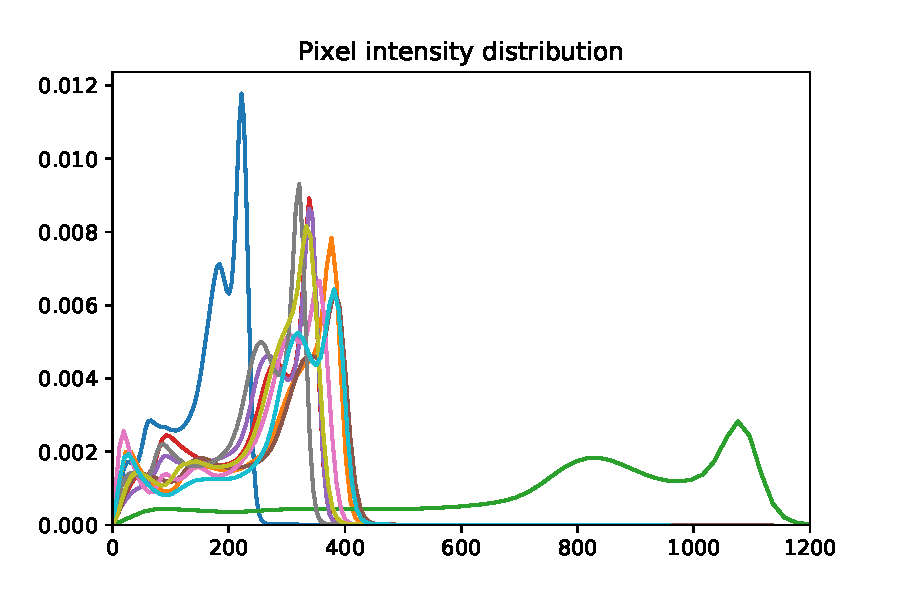
\includegraphics[width=1\linewidth]{figures/preprocessing/intensity_before_norm.pdf}
  \caption{Before voxel intensity normalization}
  \label{fig:before_intensity_normalization}
\end{subfigure}%
\begin{subfigure}{.5\textwidth}
  \centering
  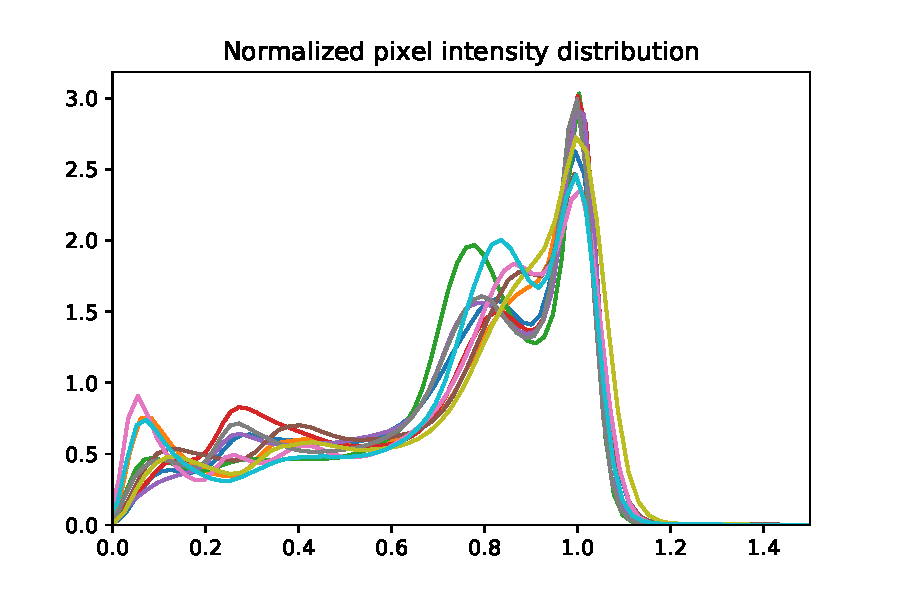
\includegraphics[width=1\linewidth]{figures/preprocessing/intensity_after_norm.pdf}
  \caption{After voxel intensity normalization}
  \label{fig:after_intensity_normalization}
\end{subfigure}
\caption{Voxel intensity distributions of 10 randomly chosen samples from the OASIS dataset.}
\label{fig:intensity_normalization}
\end{figure}

During the N4 bias correction step, we took care of uniforming the intensity of a given tissue across the whole image. The goal of this step is to do the same but across the whole dataset. To do so we will detect the intensity of a white matter voxel and set it to one. We can see in figure~\ref{fig:before_intensity_normalization} how much the intensity of the voxels can vary from two samples taken by different machines. The output of the normalization as shown in figure~\ref{fig:after_intensity_normalization} is now much more uniform across machines and therefore less prone to overfitting.

\begin{figure}
    \centering
    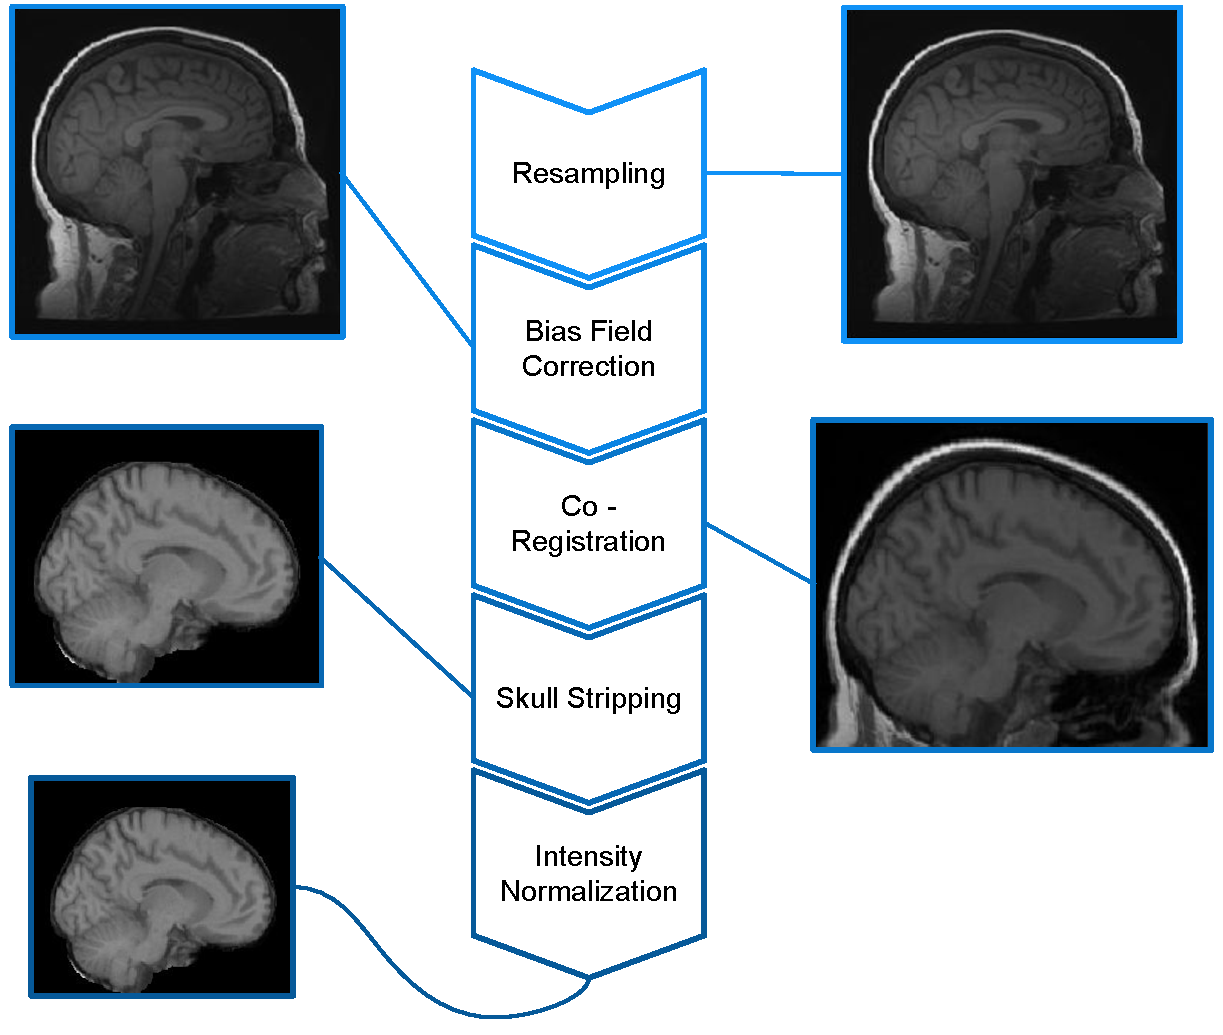
\includegraphics[width=1.0\textwidth]{figures/preprocessing/pipeline.pdf}
    \caption{Preprocessing pipeline and its outputs after each steps.}
    \label{fig:pipeline}
\end{figure}


\section{Data augmentation}

\begin{figure}
\centering
\begin{subfigure}{.4\textwidth}
  \centering
  
\includegraphics[width=1\linewidth]{figures/preprocessing/elastic_transform_input.png}
  \caption{Input grid}
  \label{fig:input_elastic_transform}
\end{subfigure}%
\hfill
\begin{subfigure}{.4\textwidth}
  \centering
  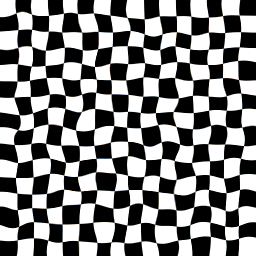
\includegraphics[width=1\linewidth]{figures/preprocessing/elastic_transform.png}
  \caption{transformed grid}
  \label{fig:output_elastic_transfor}
\end{subfigure}
\caption[Elastic]{Example\footnotemark{} of the elastic transformation applied to a grid (with alpha=991, sigma=8).}
\label{fig:elastic_transform}
\end{figure}

Data augmentation is an extra step of the training pipeline that is done right after the data has been preprocessed. One technique to overcome overfitting is to create new training samples for which we already know the labels. This trick can be applied to any type of data, but it is often used when dealing with pictures. Usually one applies a transformation to the input image, such that the model activity changes when the newly generated image is shown to it, but the transformation should be labels invariant. 
For example, it is known that CNN are translation equivariant, but not equivariant to rotations. Therefore AI expert often apply small random rotation to the image in order to augment their training set. Note that the transformation applied should be chosen carefully, as for example when dealing with a dataset such as MNIST if a rotation of more than 90 degrees is applied, it might become impossible for the network to distinguish between a rotated $6$ and a rotated $9$. 
In our case, we choose to apply random noise, small voxel intensity variation, flipping, small rotation and elastic transform. Figure~\ref{fig:data_augmentation_example} shows the different effect of the transformation on a brain scan.

\footnotetext{\href{https://gist.github.com/erniejunior/601cdf56d2b424757de5}{https://gist.github.com/erniejunior/601cdf56d2b424757de5}}
While most of the transformation applies are common, the elastic one is less known. It consists of applying a smooth deformation to the image. Figure~\ref{fig:elastic_transform} illustrates this transformation on a grid.


\begin{figure}
    \centering
    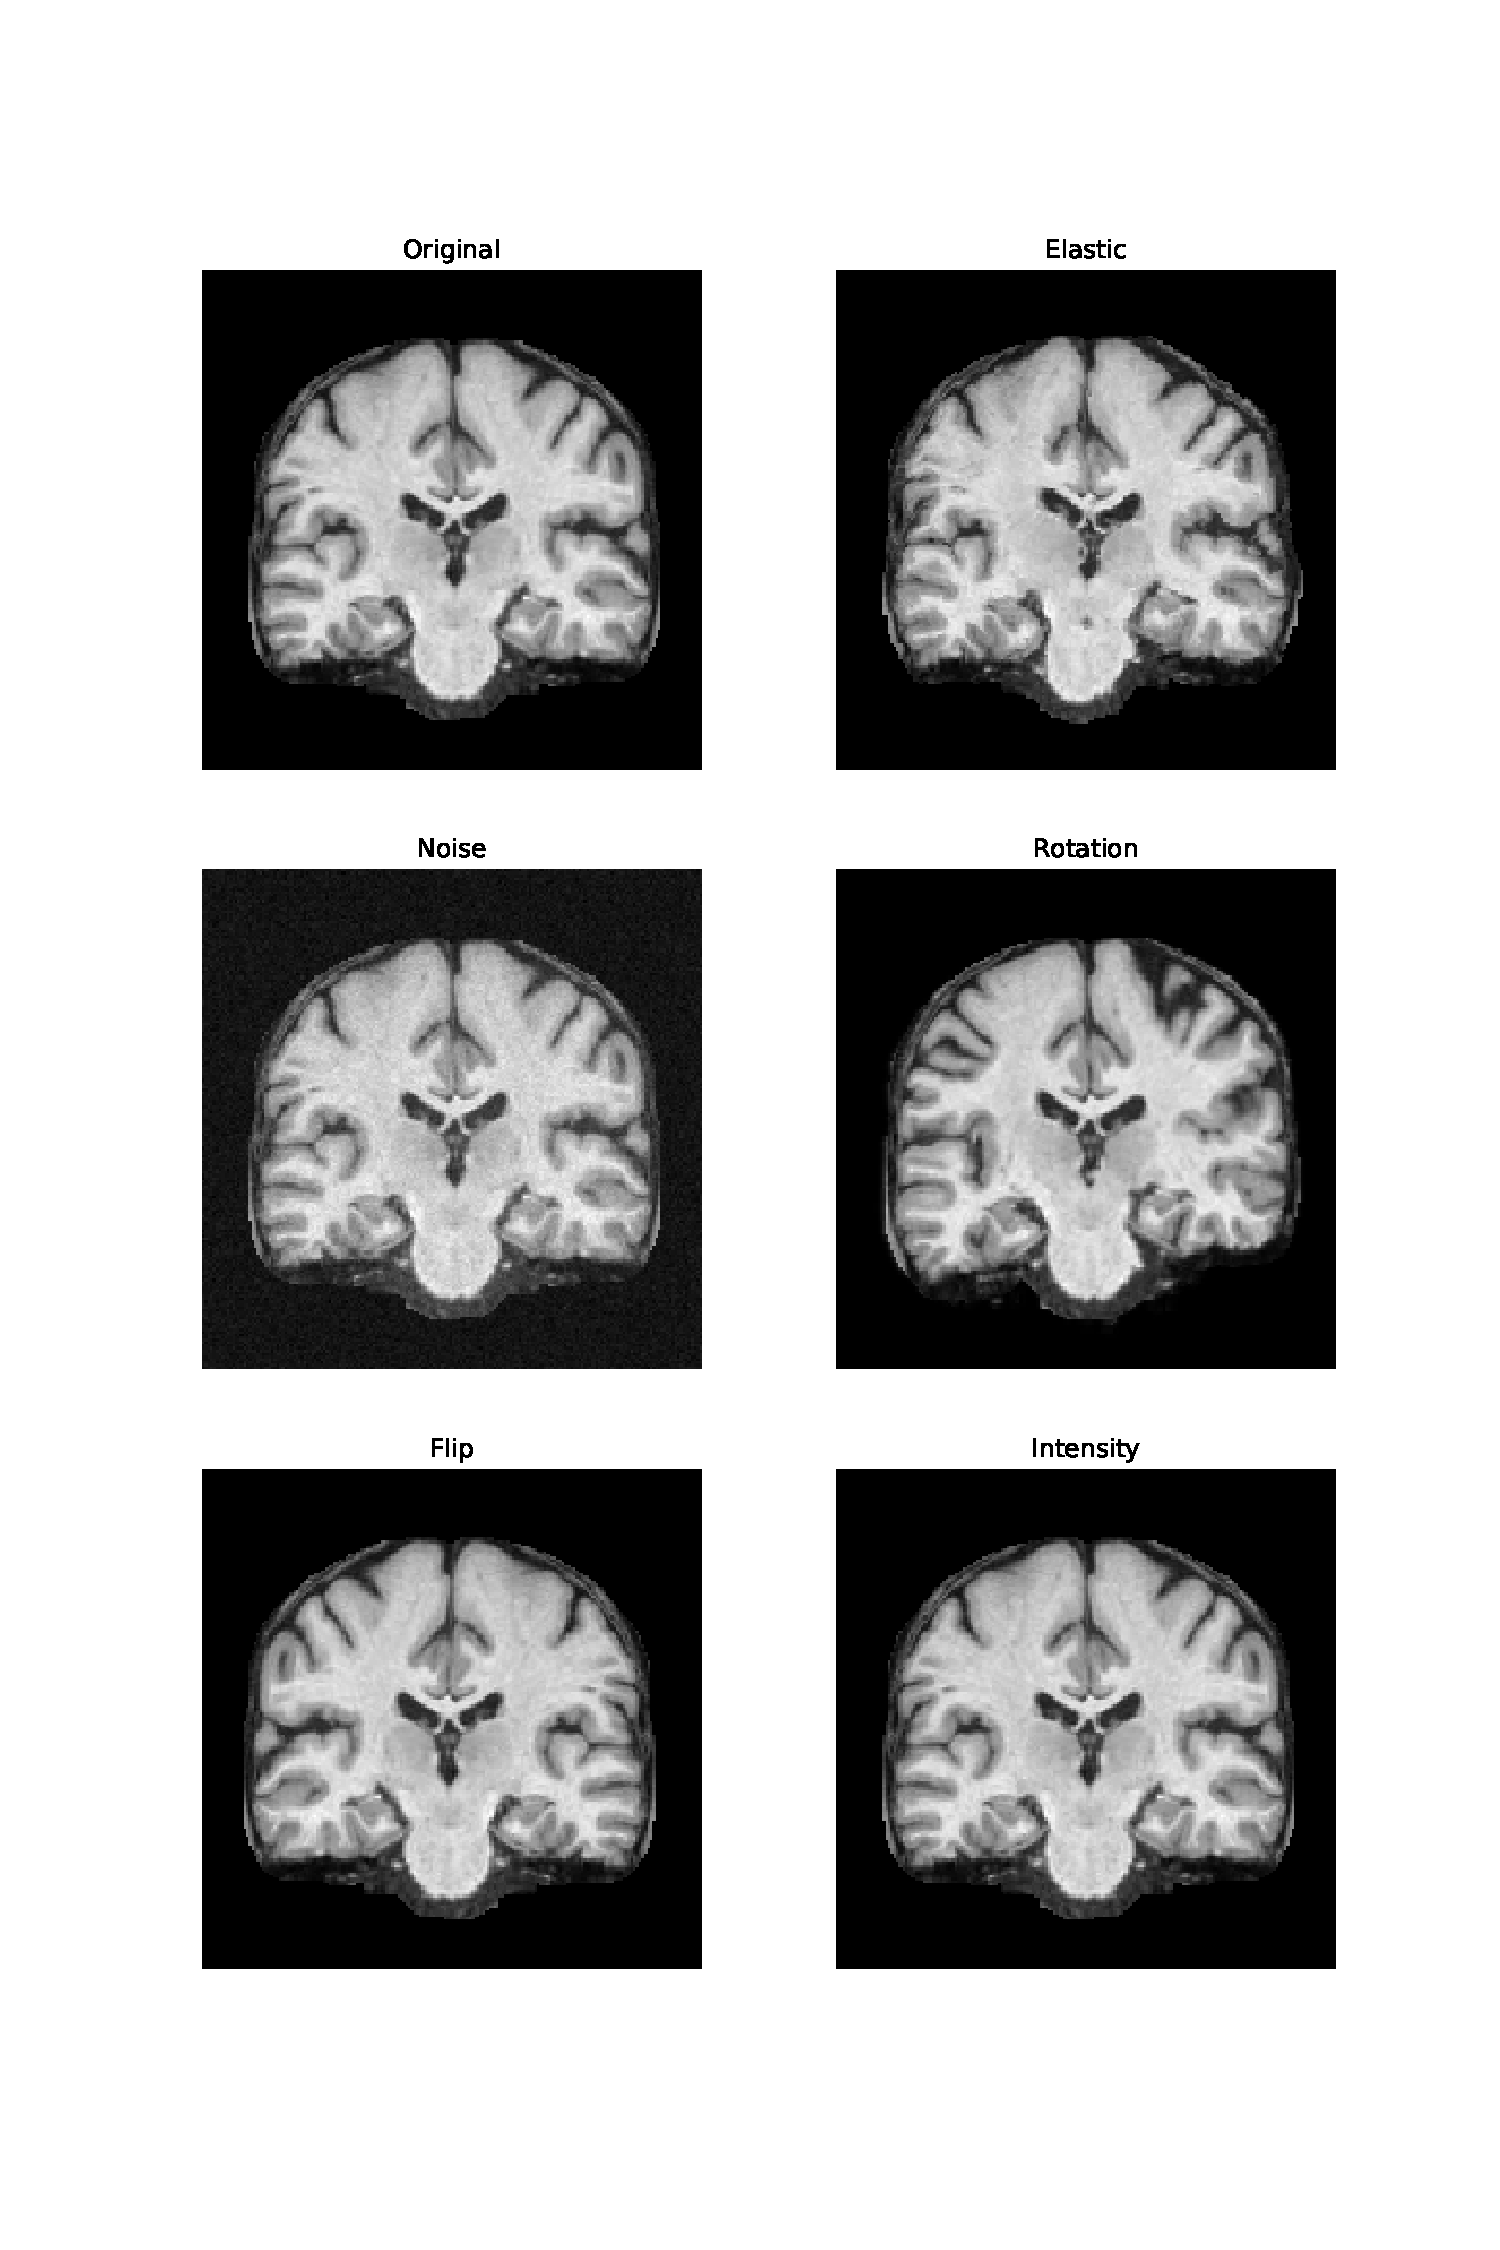
\includegraphics[width=1.0\textwidth]{figures/dataset/data_augmentation_example.pdf}
    \caption{Examples of applying data augmentation to a sample brain.}
    \label{fig:data_augmentation_example}
\end{figure}
